\documentclass{fast_latex}

% yay! We can use any kind of funky diacritic:
\usepackage[utf8]{inputenc}

\usepackage{lastpage}
\usepackage{setspace}
\usepackage{graphicx}
\usepackage[pdfborder={0 0 0}]{hyperref}		% turn on when latex is used (not miktec)
\usepackage{url} % LEO: urls \url{}
\usepackage{verbatim} % code and comment
\usepackage{longtable}
\usepackage{xspace}   % whitespace after a macro if no punctuation after the macro
\usepackage{multirow}
\usepackage{colortbl}
\usepackage{longtable}
\usepackage{array}
\usepackage{amssymb} 
\parindent0pt

\newcommand\deliverableNumber{D4.3.2}
\newcommand\deliverableTitle{Mechanisms for Gadget-Service Connections and Gadget Functionality}
\newcommand\deliverableTitleShort{Mechanisms for Gadget-Service Connections}
\newcommand\workpackageNumber{4}
\newcommand\workpackageTitle{Visual composition of screen-flow resources and interoperability with back-end Web Services}
\newcommand\authorOne{Ismael Rivera (NUIG)}
\newcommand\authorTwo{Albert Zündorf (UniKas)}
\newcommand\authorThree{Knud M\"oller (NUIG)}
\newcommand\authorFour{Author 4}
\newtheorem{example}{\emph{Example}}

\begin{document}
% explicit hyphenations
%\hyphenation{RDF-Re-po-si-to-ry}
%\hyphenation{name-space}

%\fontfamily{tahoma}\selectfont
\def\note#1{\marginpar{\footnotesize#1}} % use this to show the notes in the document
%\def\note#1{} % use this to hide the notes



%%%%%%%%%%%%%%%%%%%%%%%%%%%%%%%%%%%%%%%%%%%%%%%%%%%%%%%%%%%%%%%%%%%%%%%%%%%%%%%%
% TITLE PAGES 
%%%%%%%%%%%%%%%%%%%%%%%%%%%%%%%%%%%%%%%%%%%%%%%%%%%%%%%%%%%%%%%%%%%%%%%%%%%%%%%%
\thispagestyle{empty}

\pagenumbering{roman}

\begin{flushright}
	
\includegraphics[width=3cm]{images/FP7_logo}
\end{flushright}

\vspace{1cm}

%\begin{minipage}[p]{15cm}
	\begin{center}
		
\includegraphics{images/FAST_logo}\\
		\vspace{1cm}
		{\LARGE{\sffamily \emph{FAST AND ADVANCED STORYBOARD TOOLS}}}\\
		\vspace{0.5cm}
		{\LARGE \sffamily \emph{FP7-ICT-2007-1-216048}}\\
		\vspace{0.5cm}
		{\LARGE \sffamily \emph{http://fast.morfeo-project.eu}}\\
		\vspace{4cm}
		{\LARGE \sffamily \textbf{Deliverable \deliverableNumber}}\\
		\vspace{0.5cm}
		{\LARGE \sffamily \textbf{\deliverableTitle}}\\
		\vspace{2cm}
		{\large \sffamily \authorOne}\\
		{\large \sffamily \authorTwo}\\
		{\large \sffamily \authorThree}\\
		\vspace{0.5cm}
		\vfill
		{\large \sffamily Date: 27/02/2010}\\
		\vspace{1cm}
		{\sffamily FAST is partially funded by the E.C. (grant code: FP7-ICT-2007-1-216048).}
		
	\end{center}
%\end{minipage}


\clearpage
%%%%%%%%%%%%%%
% NEXT PAGES %
%%%%%%%%%%%%%%
\pagestyle{scrheadings}

\lohead{
\includegraphics[width=4cm]{images/FAST_logo_transparent}}
%\cohead{\small\textcolor{fast@lightgrey}{\deliverableTitle}}
%\rohead{\small{\today}}
%\lofoot{\small\textcolor{fast@lightgrey}{Task Force Ontologies}}
\cofoot{\small{FAST 216048 --- \deliverableTitleShort}}
\rofoot{\small{\thepage}}

\newpage
%
%\section*{Authors}
%\authorOne \\
%%\authorTwo \\
%%\authorThree\\
%%\authorFour\\
%
%
%\vfill
%%\section*{Project Co-ordinator}
%%\hspace*{-2,5cm}\begin{minipage}[p]{14cm}
%%Dr. Ansgar Bernardi \\
%%German Research Center for Artificial Intelligence (DFKI) GmbH \\
%%Trippstadter Strasse 122 \\
%%D 67663 Kaiserslautern \\
%%Germany \\
%%Email: bernardi@dfki.uni-kl.de, phone: +49 631 205 3582, fax: +49 631 205 4910 \\
%%\end{minipage}
%
%
%\section*{Partners}
%Telef\'onica Investigaci\'on y Desarrollo (Telef\'onica I+D), Spain \\
%National University of Ireland, Galway (NUIG), Republic of Ireland \\
%Kassel University, Germany \\
%Cyntelix Corporation, Republic of Ireland \\
%SAP AG, Germany \\
%Universidad Polit\'ecnica de Madrid (UPM), Spain
%
%
%\vspace{0.3cm}
%\begin{footnotesize}
%Copyright: FAST Consortium 2009\\
%\end{footnotesize}

%\clearpage


\section*{Version History}

\begin{small}
\begin{tabular}{|l|l|l|p{7.5cm}|}
\hline
\rowcolor{fast@lightgrey}\textcolor{white}{\textbf{Rev. No.}} &
                            \textcolor{white}{\textbf{Date}} &
                            \textcolor{white}{\textbf{Author (Partner)}} &
							\textcolor{white}{\textbf{Change description}}\\ \hline
%0.1 & 15.12.2008 & Knud M\"oller (NUIG) & template modelled \\ \hline
%0.2 & 15.02.2009 & Knud M\"oller (NUIG) & content moved from wiki after internal review \\ \hline
1.0 & 26.02.2010 & Ismael Rivera (NUIG), & Final version ready for external review \\ 
 & & Albert Zündorf (UniKas) & \\ \hline
2.0 & 27.02.2011 & Ismael Rivera (NUIG), & Final version ready for external review \\ 
 & & Albert Zündorf (UniKas) & \\
 & & Knud M\"oller (NUIG) & \\ \hline
\end{tabular}
\end{small}

\color{black}

\vfill
%{\bf Explanations of abbreviations on front page}\\
%\\
%%Nature \\
%R: Report \\
%P: Prototype \\
%R/P: Report and Prototype \\
%O: Other \\
% \\
%Dissemination level \\
%PU: Public \\
%PP: Restricted to other FP6 participants \\
%RE: Restricted to specified group \\
%CO: Confidential, only for NEPOMUK partners \\

\newpage

%%%%%%%%%%%%%%%%%%%%%
% Executive Summary %
%%%%%%%%%%%%%%%%%%%%%

\clearpage

\section*{Executive Summary}
\doublespacing

This deliverable exposes several mechanisms which will allow the connection and interaction between end-user's interfaces to third-party back-end services.

These back-end services cannot be directly used; hence they need to be encapsulated in what in the FAST platform is called Resource Adapters. The application of semantics to the back-end, through the corresponding Resource Adapters, and front-end building blocks assures a powerful instrument in the task of building new gadgets, improving the search, and enhancing the connection among the different building blocks which compose a gadget.

Therefore, the focus of this deliverable is to define how these wrappers will be constructed to allow the FAST platform exploiting web services \cite{GustavoAlonso2003} such as RESTful web services, SOAP-based web services and semantic web services through WSMO, and define mechanisms to connect them within the gadgets.

\newpage

%%%%%%%%%%%%%%%%%%%%%
% Document Summary %
%%%%%%%%%%%%%%%%%%%%%

\clearpage

\section*{Document Summary}
% double spacing from here on:
\singlespacing
\begin{small}

\begin{tabular}
	%{| >{\columncolor{fast@lightgrey}}p{3.25cm}|p{6cm}|p{2cm}|p{2cm}|}
	{| >{\columncolor{fast@lightgrey}}p{3.25cm}|p{6cm}|p{2cm}|p{2cm}|}
	\hline
	\textcolor{white}{\textbf{Code}} & {FP7-ICT-2007-1-216048} & {\textbf{Acronym}} & {FAST}\\ \hline
	\textcolor{white}{\textbf{Full title}} & \multicolumn{3}{l|}{Fast and Advanced Storyboard Tools}\\ \hline
	\textcolor{white}{\textbf{URL}} & \multicolumn{3}{l|}{\url{http://fast.morfeo-project.eu}}\\ \hline
	\textcolor{white}{\textbf{Project officer}} & \multicolumn{3}{l|}{Annalisa Bogliolo}\\ \hline
\end{tabular}

\vspace{0.5cm}

\begin{tabular}
	{| >{\columncolor{fast@lightgrey}}p{3.25cm}|p{1.25cm}|p{1cm}|p{1cm}|p{6.32cm}|}
	\hline
	\textcolor{white}{\textbf{Deliverable}} & {\textbf{Number}} & {\deliverableNumber} & {\textbf{Name}} & {\deliverableTitle}\\ \hline
	\textcolor{white}{\textbf{Work package}} & {\textbf{Number}} & {\workpackageNumber} & {\textbf{Name}} & {\workpackageTitle}\\ \hline
\end{tabular}

\vspace{0.5cm}

\begin{tabular}
	{| >{\columncolor{fast@lightgrey}}p{3.25cm}|p{1.4cm}|p{3.28cm}|p{1.6cm}|p{3.29cm}|}
	\hline
	\textcolor{white}{\textbf{Delivery data}} & {\textbf{Due date}} & {28/02/2011} & {\textbf{Submitted}} & {27/02/2011}\\ \hline
	\textcolor{white}{\textbf{Status}} & \multicolumn{2}{l|}{} & \multicolumn{2}{l|}{final}\\ \hline
	\textcolor{white}{\textbf{Dissemination Level}} & \multicolumn{4}{l|}{Public $\boxtimes$ / Consortium $\square$}\\ \hline
	\textcolor{white}{\textbf{Short description of contents}} & \multicolumn{4}{p{10.85cm}|}{D4.3.2 is...}\\ \hline
	\textcolor{white}{\textbf{Authors}} & \multicolumn{4}{l|}{\authorOne, \authorTwo, \authorThree}\\
%	{} & \multicolumn{4}{l|}{}\\ 
%	{} & \multicolumn{4}{l|}{}\\ 
%	{} & \multicolumn{4}{l|}{}\\
	\hline
	\textcolor{white}{\textbf{Deliverable Owner}} & \multicolumn{2}{l|}{\authorOne} & \textbf{email} & {ismael.rivera@deri.org} \\ \cline{4-5}
	\textcolor{white}{\textbf{(Partner)}} & \multicolumn{2}{l|}{} & \textbf{phone} & {+353 91 ?????} \\ \hline
	\textcolor{white}{\textbf{Keywords}} & \multicolumn{4}{p{10.85cm}|}{FAST, web services, WSDL, REST, SOAP, WSMO}\\ \hline
\end{tabular}
\end{small}
\newpage

%%%%%%%%%%%%%%%%%%%%%
% TABLE OF CONTENTS %
%%%%%%%%%%%%%%%%%%%%%
\doublespacing
\setcounter{tocdepth}{3}
\tableofcontents
\cleardoublepage
\pagenumbering{arabic}

%%%%%%%%%%%%%%%%%%%%%%%%%
% BEGINNING OF SECTIONS %
%%%%%%%%%%%%%%%%%%%%%%%%%

\clearpage
\rofoot{\small{Page \thepage\ of \pageref{LastPage}}}

\section{Introduction} % (fold)
\label{sec:introduction}

\subsection{Goal and Scope} % (fold)
\label{sub:goal_and_scope}

The objective of this deliverable is the analysis and development of mechanisms to facilitate the connection between screen-flow gadgets and underlying Web services, based on front-end user requirements and on the semantic descriptions of the service wrappers, and to develop these service wrappers from of the Web services' APIs and formal descriptions.

% subsection goal_and_scope (end)

\subsection{Structure of the Document} % (fold)
\label{sub:structure_of_the_document}

This deliverable is structured as follows. Section~\ref{sec:introduction} states the goal, scope and structure of the document. Section~\ref{sec:web_services_wrapping} describes what a service wrapper is, how the platform is able to interact with web services, how these wrappers are build and then discovered to be reused in any gadget. Finally, Section~\ref{sec:restful_web_services_wrapper_tool} defines the service wrapper tool built to facilitate FAST users to create Resource Adapters of RESTful web services.

% subsection structure_of_the_document (end)

\subsection{Changes from Previous Version} % (fold)
\label{sub:changes_from_previous_version}

\textcolor{red}{To be done...}


% subsection changes_from_previous_version (end)

% section introduction (end)

\clearpage
\section{Web Services Wrapping} % (fold)
\label{sec:web_services_wrapping}

In the context of FAST philosophy, a service is a software element or system, often deployed within enterprise boundaries, designed to support interoperable Machine-to-Machine interaction over a network (e.g. Web Services, Databases, CORBA or RPC interfaces...). These services have to be used by the gadgets, but there are several complications to be resolved in order to communicate the front-end (i.e. the gadget user interface and logic) with those services, such as the disparity of interfaces and invocation mechanisms. Another issue is the complexity for an end-user to interact with those services. Hence, this interaction will be shift to a user-interaction paradigm through a user-friendly graphical interface (service front-end), allowing both humans and machines to interact with the services through a uniform fashion.

Therefore, a complex gadget in terms of FAST is aimed to provide a functional access from a graphical user interface to a set of services (SOAP or REST-based Web services) and data sources (Atom/RSS feeds). These services and data sources need to be modelled and encapsulated within the platform in order to allow the discovery and use of them by other components (i.e. forms and operators). This is called Resource Adapter in the FAST platform. Figure~\ref{fig:complex_gadget_architecture} illustrates their position and interaction with the rest of the building blocks within a gadget.

\begin{figure}
  \begin{center}
    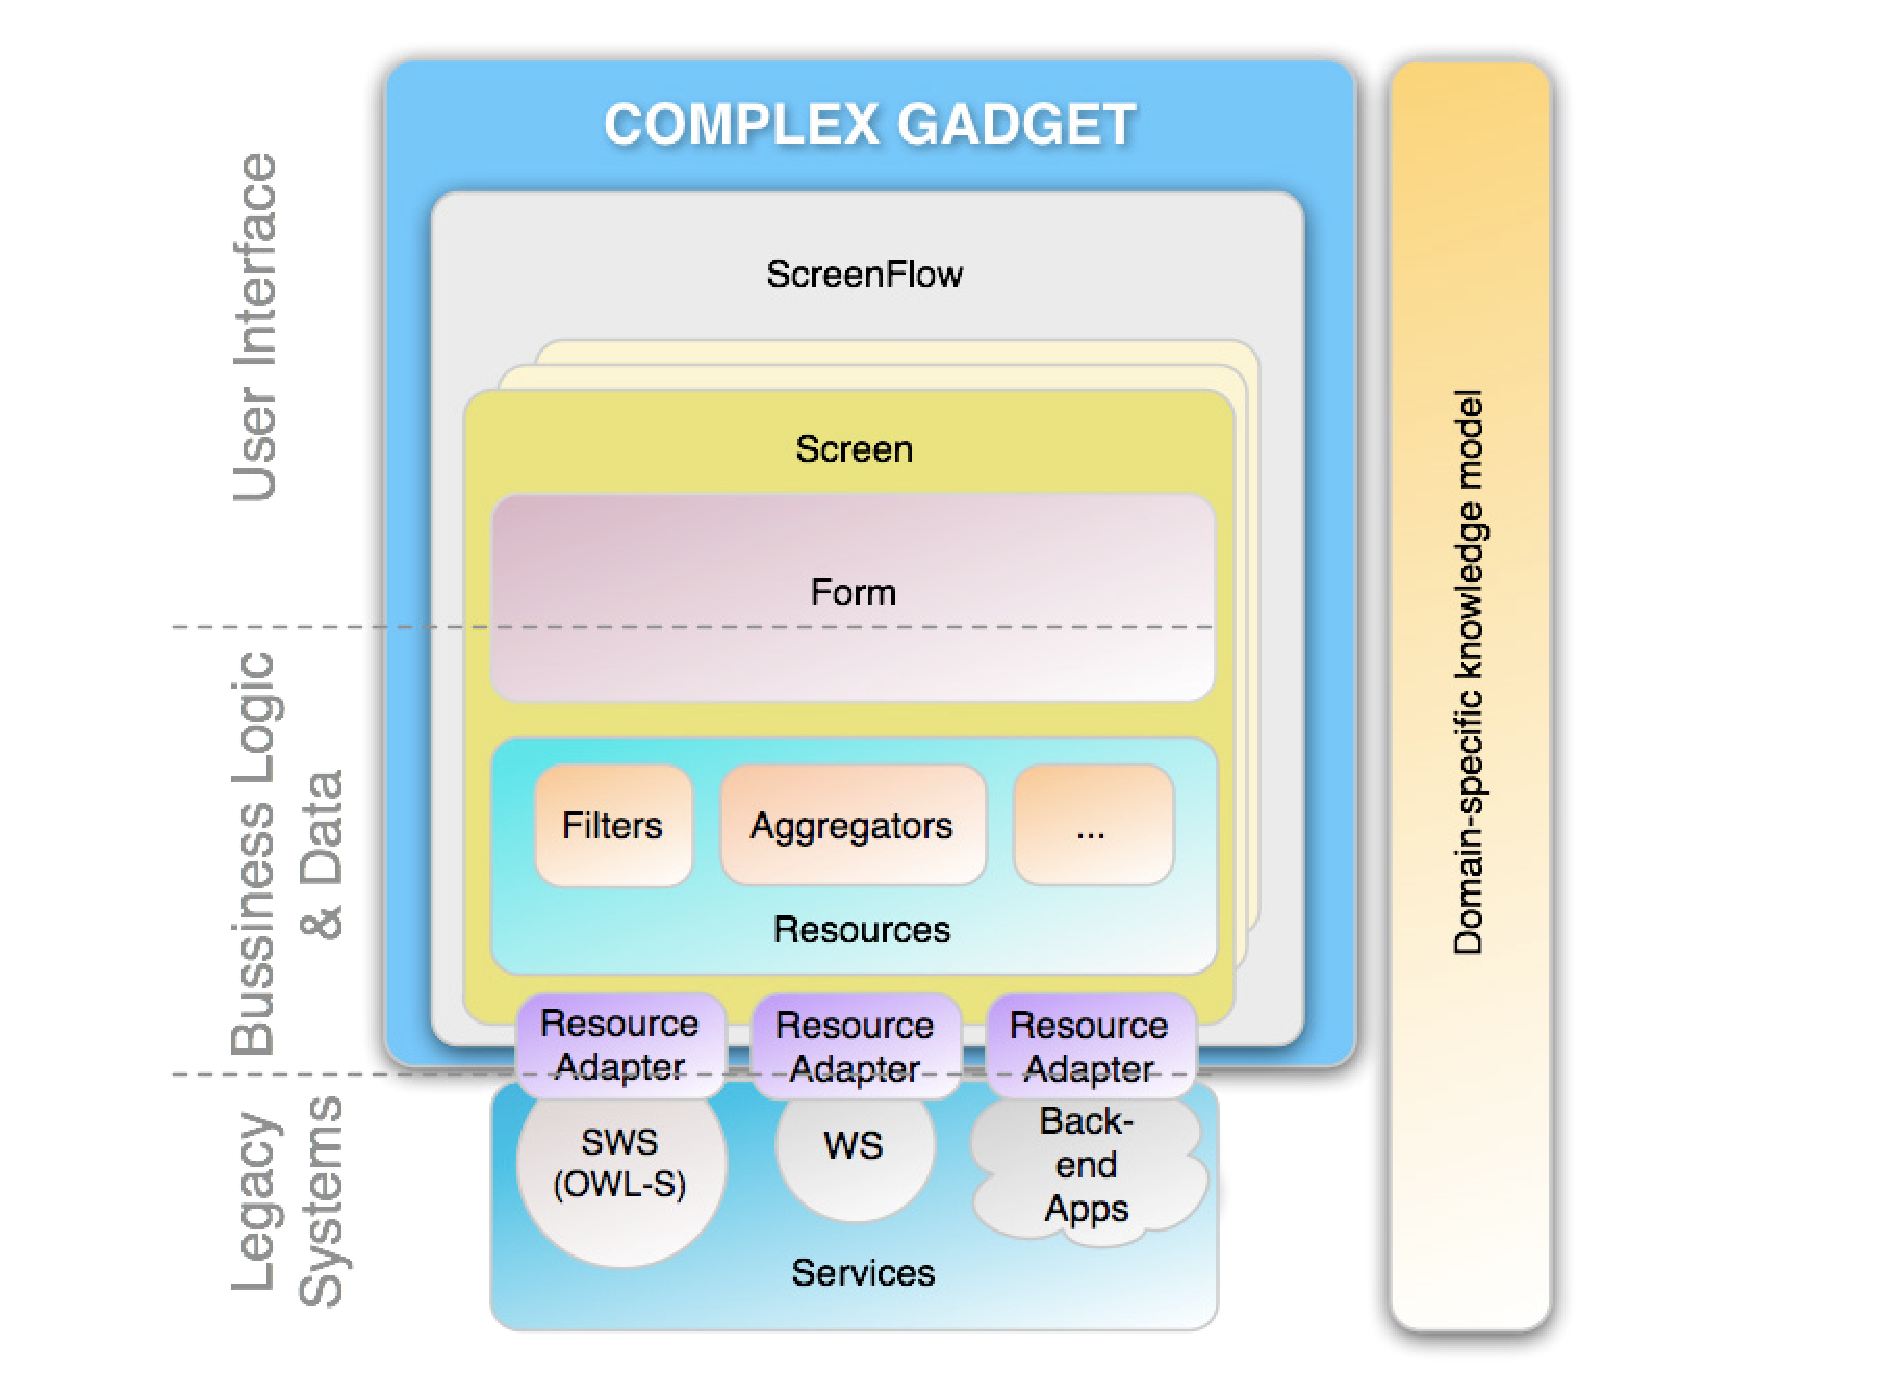
\includegraphics[width=\linewidth]{images/ComplexGadgetArchitecture.pdf}
    \caption{Complex Gadget Architecture}
    \label{fig:complex_gadget_architecture}
  \end{center}
\end{figure}

Once a brief background has been shown, the following sections explain how a user, in this case a resource developer, can build Resource Adapters, and how another user, a screen developer for instance, will discover and connect them while creating a screen. Hence, these three phases are called: building, discovery and connection.

\subsection{Building} % (fold)
\label{sub:building}

\subsubsection{REST-based Web Services} % (fold)
\label{ssub:rest_based_web_services}

REST is a term to describe an architecture style, not a standard, of networked systems. The acronym REST stands for Representational State Transfer. REST-based or RESTful web services \cite{Fielding2000} are created identifying all of the conceptual entities or resources which want to be exposed as services. Those entities or resources should be nouns, not verbs (orders, tickets, etc.). Then, the interaction with those resources is made by convention using HTTP verbs such as GET, POST, PUT or DELETE, in order to retrieve, create, modify or delete them.

REST is lightweight (not a lot of extra xml markup, human readable results), but unlike SOAP-based web services, which have a standard vocabulary, and commonly used, to describe the web service interface through WSDL, RESTful web services are currently not formally described most of the times. For a service consumer to understand the context and content of the data that must be sent to and received from the service, both the service consumer and service producer must have an out-of-band agreement. This takes the form of documentation, sample code, and an API that the service provider publishes for developers to use. For example, the many web-based services available from Google, Yahoo, Flickr, Amazon, and so on have accompanying artefacts describing how to consume the services. This style of documenting REST-based web services is fine for use by developers, but it averts tools from programmatically consuming such services and generating artefacts specific to programming languages, as a web service described using WSDL allows. Nevertheless, Web Application Description Language (WADL) attempts to resolve some of these issues by providing a means to describe services in terms of schemas, HTTP methods, and the request or response structures exchanged, but this language is not widely adopted yet by RESTful web service developers.

To permit a high number of REST-based web services to be integrated to the FAST platform, the approach taken is from a manual development perspective. There is no need of a formal document such as WADL defining the web service, for this reason, building service wrappers for these services involve the correct understanding of the service by a human being and a tool to facilitate this task. This tool is explained in detail in Section~\ref{sec:restful_web_services_wrapper_tool}.

% subsubsection rest_based_web_services (end)

\subsubsection{SOAP Web Services} % (fold)
\label{ssub:soap_web_services}

SOAP-based web Services or "Heavyweight Web Services" use Extensible Markup Language (XML) \cite{XML1.1} messages that follow the Simple Object Access Protocol (SOAP) standard \cite{SOAP1.2} and have been popular with traditional enterprise, usually relying on HTTP for message negotiation and transmission. In such services, there is often a machine-readable description of the operations offered by the service written in a Web Services Description Language (WSDL) document. Hence, the advantage of using WSDL is that it can be programmatically processed. 

Shortly, a WSDL definition of a service, regarding the WSDL 2.0 specification \cite{WSDL2.0}, will contain the following information:
\begin{description}
	\item[Interfaces] A set of Interface components describing sequences of messages that a service sends and/or receives.
	\item[Bindings] A set of Binding components describing concrete message formats and transmission protocols which may be used to define the endpoints.
	\item[Services] A set of Service components describing a set of endpoints at which a particular deployed implementation of the service is provided.
	\item[Element declarations] A set of Element Declaration components defining the name and content model of the element information items such as that defined by an XML Schema global element declaration.
	\item[Type definitions] A set of Type Definition components defining the content model of the element information items such as that defined by an XML Schema global type definition.
\end{description}

From a specific WSDL definition, a set of methods or operations can be easily extracted which encloses a set of inputs and outputs. These operations would be transformed into actions, and the inputs and outputs would be used to define Resource Adapter pre-/post-conditions. With the use of this information along with the XML Schema defining the types, a Resource Adapter can be semantically defined.

To integrate WSDL defined services into the FAST platform, we again propose an interactivce approach: We extend the tool for REST service wrapping with the ability of loading WSDL definitions of a service and this WSDL definition is then exploited for guidance of the user through the Resource Adapter construction, cf. Section~\ref{sec:restful_web_services_wrapper_tool}.

% subsubsection soap_web_services (end)

\subsubsection{WSMO Web Services} % (fold)
\label{ssub:wsmo_web_services}

Semantic web services bring a number of advantages in the creation of the resources adapters over classic web services. Formal and semantic descriptions of web services allow mechanisms to raise its exploitation in a more automatic way. In this section, some general notions of the Web Service Modelling Ontology (WSMO) will be explained and how FAST can make use of it.

In a few words, WSMO provides means to describe all relevant aspects of semantic web services in a unified manner. A web service description in WSMO consists of five sub-components: non-functional properties, imported ontologies, used mediators, a capability and interfaces. However, we will focus on the capabilities and the interfaces since they are components which will make possible the integration of these services in FAST.

Capabilities and interfaces are the two types of Web Service description in WSMO. The capabilities describe the different functions of WSMO, while the interfaces specify:
\begin{enumerate}
	\item How to communicate with a web service in order to avail of its functionality. This is called Choreography.
	\item How the functionality of a web service is enabled by interacting with other Web Services. This is called Orchestration.
\end{enumerate}

A web service in WSMO defines one and only one capability. The capability of a web service defines its functionality in terms of pre-/post-conditions, assumptions and effects. A web service capability is defined by specifying the following elements: non-functional properties, imported ontologies, used mediators, shared variables, pre-condition, post-condition, assumption, and effect.

Basically, the web service will offers to a client a post-condition when some conditions are met in the information space (pre-condition). Effects and assumptions can stay out of this study, since they will not be taken into account by any of the building blocks of a gadget.

Like WSDL defined services, we incorporate WSMO services into the FAST platform in an interactive storyboard driven approach. The FAST tool described in Section~\ref{sec:restful_web_services_wrapper_tool} reads the WSMO specification of a service and exploits this information again for guidance for the construction of a Resource Adapter. 

% subsection building (end)

\subsection{Discovering} % (fold)
\label{sub:discovering}

In the building phase, every Resource Adapter is created sharing a common structure for screen components, such as forms, operators and resources. Hence, it will have a set of actions which will contain a set of pre-conditions to satisfy in order to be executed, and after its execution, it may produce any of the conditions of their post-conditions.

For this reason, a screen developer during the screen development phase is able to reuse these screen components which are already stored in the Catalogue, establishing which the screen's pre-/post-conditions are, and then the system will suggest several screen components which may satisfy these pre-/post-conditions. In a first step, the system will suggest screen components which have any of the pre-conditions which can be connected to any of the screen pre-conditions (the connection will be represented by an internal pipe), and the same would happen for the post-conditions. Once a screen component is inserted into the screen, the system will take its definition (screen components, pipes, etc.) into consideration to recommend new screen components which can be connected to the ones the screen is composed of.

For a further explanation on how the recommendation algorithms are implemented, please see~\cite{rivera2011catalogue_user_manual}.

% subsection discovery (end)

% section web_services_wrapping (end)


\clearpage
\section{Service Wrapper Tool} % (fold)
\label{sec:restful_web_services_wrapper_tool}

In FAST, the Service Wrapper Tool will be in charge of the Resource Adapters' building phase. The building of resource adapters is done in three steps: in a first step, we define which pre- and post-conditions are used to pass parameters between FAST building blocks and the resource adapter. The second step is in charge of the construction of a service request and the third step analyses the response got from the execution of the service, allowing the extraction of facts contained in that response and mapping them to domain-specific classes or concepts from the ontologies used within FAST by the building blocks' conditions.


\subsection{Defining pre- and post-conditions} % (fold)
\label{sub:resource_adapter_parameters}

We will demonstrate the use of the Service Wrapper Tool on the example of a simple \emph{Formula1} service. In the first tab of the Service Wrapper Tool, the user defines the name and the pre- and post-conditions of the desired Resource Adapter, cf. Fig. \ref{fig:construct_pre_post_conditions}. For the pre-condition, we provide a name, a type, and an example value. The type of a pre- or post-condition is chosen from a drop down list of available concepts. The list of available concepts, together with its properties and some example data (instances) is retrieved from the Catalogue. The example value is used for test requests during subsequent construction steps. We keep track of example values provided for different domain concepts and propose them, when the domain concept is re-used e.g. in another Resource Adapter. 

\begin{figure}
  \begin{center} 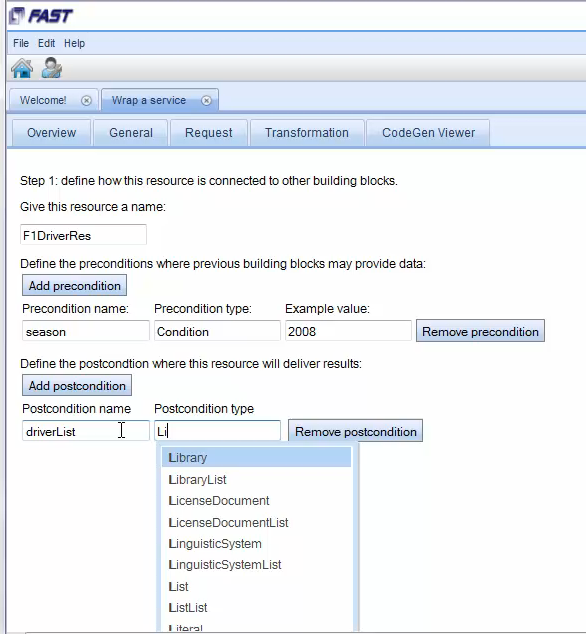
\includegraphics[width=\linewidth]{images/ServiceWrapperToolGVSWithPrePostConds.png}
    \caption{Configuring pre- and post-conditions of a Resource Adapter}
    \label{fig:construct_pre_post_conditions}
  \end{center}
\end{figure}


\subsection{Constructing service requests} % (fold)
\label{sub:constructing_service_requests}

In our simple case, the service request consists just of a URL that is easily retrieved from API documentation page of our Formula1 service. This URL consists of the service address \url{http://ergast.com/api} followed by the year we are querying for followed by the category \verb|drivers| we are interested in. The user may grab such an URL from the API documentation page of the targeted web service and drop it into the Request tab of the Service Wrapper Tool, cf. Figure~\ref{fig:construct_service_request}. The Service Wrapper Tool will than analyze the dropped URL and split it into its parts and provide a convenient form allowing to edit e.g. all the parameters of the URL. In our example the URL has no parameters so the parameter form shows only the base URL. 

For WSDL or WSMO services, the Service Wrapper Tool provides additional support for the construction of the request. The user may point to the WSDL or WSMO definition of the targeted service. The Service Wrapper Tool then reads this definition and analyses it. With the help of this information, the Service Wrapper Tool provides interactive guidance for selecting the desired operation from a service and then it retrieves the operation descriptions and fills the request parameter form adequately.

Now we have to connect the request parameters to the parameter values passed via the pre-conditions to the Resource Adapter. In our case, we replace the year part of the URL with a placeholder for the pre-condition season \verb|<season>|, see Request URL input field at the top of Figure~\ref{fig:construct_service_request}.  

In our example, we use a simple HTTP GET request. The Service Wrapper Tool also supports the other kinds of HTTP methods as POST, PUT or DELETE. For POST requests, one usually passes parameters within a special post body. For unstructured POST bodies, we provide a text area allowing the user to fill in placeholders for references to pre-condition values. In case of structured POST bodies as in the case of WSDL and WSMO services the POST body uses a structured text format based e.g. on JSON or XML. In that case, our tool parses the body text and the user is able to adapt the parameters via the request parameter form part. This means, the user may easily use the request parameter form part to fill in pre-condition placeholders.

\textcolor{red}{WSDL is usually used with SOAP and XML, JSON wouldn't be common in this case. And from my understanding, the user has to hand-write the POST body? therefore the SOAP message? that's doable, but pretty hard and tedious. - Ismael}
\textcolor{blue}{Well as I understood, in case of WSDL the post body is structured (XML?). Thus, we parse that body, identify the key value pairs of the parameters and come up with an input form as we do for URL parameters. Easily done. 
I have changed the text above slightly to reflect this better. - Albert}
\textcolor{red}{yes and no. it uses SOAP, which relies on XML, but it's something different. the SOAP message will have more info that pre-/post-condition needs. - Ismael}


\textcolor{red}{Is PUT and DELETE supported? if so, how? - Ismael}
\textcolor{blue}{Well, it will be supported for the review meeting. Actually Dennis has done a lot of work on this and it is pretty complete. 
After all a post request looks very much like a get request. Yes, the data is provided in some body. But, the FAST API, that works as relay for us, provides a method, where you pass an url, the request kind (GET, PUT, DELETE, ...) and the parameters. Depending on the kind, this method puts the parameters either in the URL or in some body. No difference for us.}
\textcolor{red}{ok, grand!}

Figure~\ref{fig:construct_service_request} shows the screen to construct the service requests.

\begin{figure}
  \begin{center}
    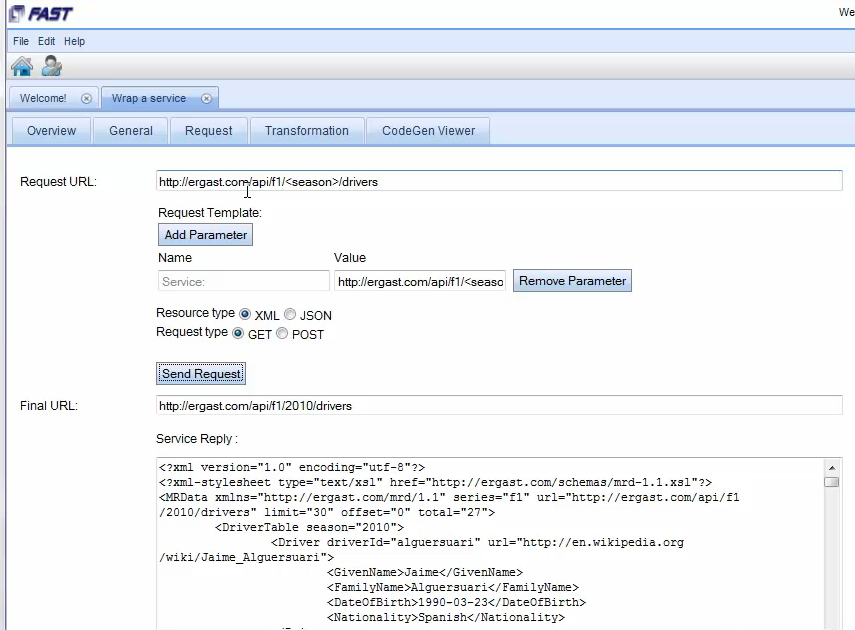
\includegraphics[width=\linewidth]{images/ServiceWrapperToolGVSRequestTemplate.png}
    \caption{Constructing the service request and its parameters}
    \label{fig:construct_service_request}
  \end{center}
\end{figure}


Below the request parameter editing form of Figure~\ref{fig:construct_service_request}, a \textit{Send Request} button allows to validate the constructed request by sending it to the specified service address (via a server relay). Then the placeholders for pre-conditions are replaced with example values and the resulting request is shown below the parameter form. In addition, the request is sent and the response is shown on the bottom of that page. This gives the user a fast feedback whether the constructed request works as desired. 

\subsubsection{Limitations} % (fold)
\label{ssub:limitations}

It is worth pointing out that currently the Service Wrapper Tool is able to construct input ports for the wrappers using just basic types. However, every building block accepts any (complex) concept as a pre-/post-condition, so the wrapper tool needs to be adapted to permit any concept as input or pre-condition, extracting the required text to construct the request. This should be easy to achieve before the project review. 

\textcolor{red}{I guess this paragraph will be rewritten...because my understanding is that we do support constructing wrappers with ``complex'' pre-/post-conditions and not just basic types. - Ismael}

% subsubsection limitations (end)

% subsection constructing_service_requests (end)

\subsection{Interpreting service responses} % (fold)
\label{sub:interpreting_service_responses}

Once the service request is constructed and sent to the service provider, it will send back a response. This response message could be serialize in any format, though the most common formats used nowadays are XML or JSON. To continue the example started in the previous section, the response of the Formula1 service will is formatted in XML. Th Service Wrapper Tool supports both JSON and XML.

\subsubsection{Translation XML/JSON into Facts} % (fold)
\label{ssub:translation_xml_into_facts}

Figure~\ref{fig:response_service_execution} shows the data tranformation tab of the wrapper tool. 

\begin{figure}
  \begin{center}
      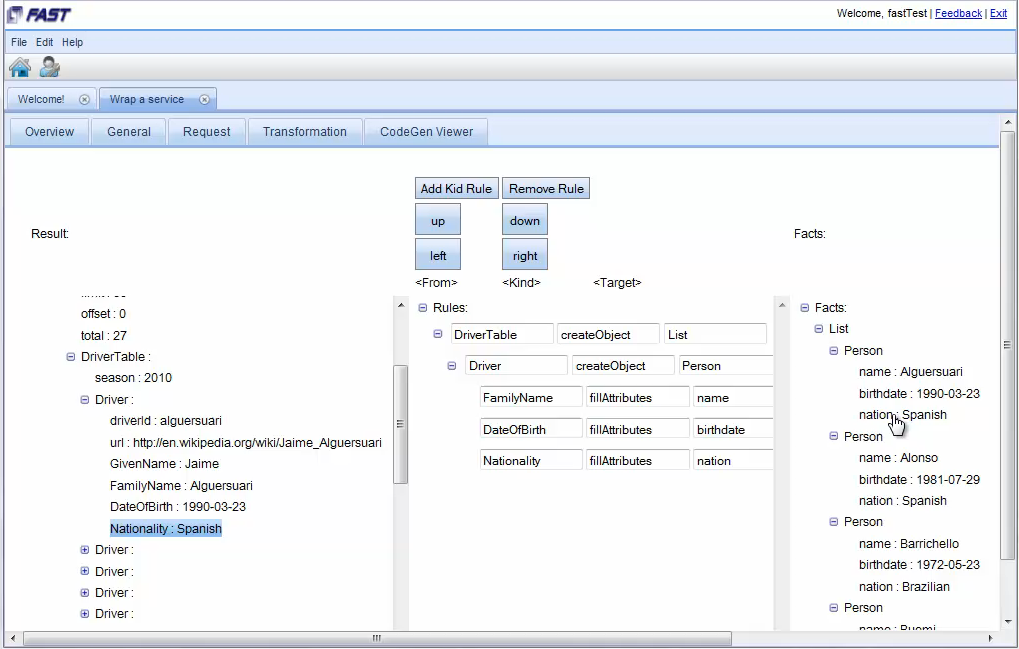
\includegraphics[angle=90,width=0.8\linewidth]{images/ServiceWrapperToolGVSWithTransformationRulesF1.png}
    \caption{Interactive, rule based transforming of an XML response to FAST facts}
    \label{fig:response_service_execution}
  \end{center}
\end{figure}

Once the service response has been retrieved, it is shown in the transformation tab as an interactive object tree, as it can be seeing on the left side of Figure~\ref{fig:response_service_execution}. To construct this interactive object tree, the XML or JSON document is parsed into a DOM, and a simplified tree representation of that DOM is built up. This tree representation of the XML/JSON data is used as an input to construct transformation rules.

A transformation rule is used to analyse the XML/JSON data and to generate domain-specific facts from concepts from the ontologies used by the pre-/post-conditions of the different building blocks. A transformation rule is composed of three elements, as the middle part of Figure~\ref{fig:response_service_execution} shows. First, the \textit{from} field indicates the XML elements to be translated by rule. These XML elements are identified by the tagname of a DOM element from the XML document. Second, the type of the rule will be set, taking one of the following values: \emph{createObject}, \emph{fillAttributes} or \emph{dummy}. And third, the target of the rule specifies a certain concept or attribute, to be created or filled. A detailed explanation of the type of actions to be triggered from the transformation rules is:
\begin{description}
	\item[action \emph{createObject}] specifies the creation of a new fact object. The type of that new fact is provided in the third compartment. In the example being explained, the root rule searches for XML elements with tagname \emph{DriverTable} and for each such element a \emph{List} fact is created. The resulting facts are shown in a facts tree in the right of Figure~\ref{fig:response_service_execution}.
	\item[action \emph{fillAttributes}] does not create a new fact but it fills the value of the attribute provided as third part of such rules. In our example, the third transformation rule searches for XML elements with tagname \emph{FamilyName}. Note, the rule is a sub-rule of the second rule, which generates \emph{Person} facts. Thus, the sub-rule searches for \emph{FamilyName} tags only in the subtree of the XML data that has been identified by an application of the parent rule before. For example, the \emph{Driver} rule may just have been applied to the first \emph{Driver} element of the XML data. Then, the \emph{FamilyName} rule is applied only to the first \emph{Driver} sub-tree of the XML data and thus it will find only one \emph{FamilyName} element in that sub-tree. The value of that \emph{FamilyName} element is then transfered to the \emph{name} attribute of the corresponding \emph{Person} fact. Actually, our \textit{from} fields allows also to refer to parts of an XML attribute e.g. to \textit{words} 1 through 3. It is also possible to combine constant text and elements of multiple XML tree elements. A \textit{from} field may also refer to multiple tags of the source tree, e.g. to combine a full name from a first name and a family name field.  
	\item[action \emph{dummy}] does not create or modify any facts but such rules are just used to narrow the search space for their sub-rules. For example, in the Amazon case, the XML data for an item contains sections for \emph{minimum price}, \emph{maximum price}, and \emph{average price}. Each such section contains the \emph{plain price} and the \emph{formatted price}. Thus, in the Amazon case, a rule that searches for \emph{formatted price} elements within an \emph{Item} element would retrieve three matches. Using a dummy rule, we may first search for \emph{minimum price} elements and then search for \emph{formatted price} elements within that sub-tree.
\end{description}

Since FAST is storyboard oriented, the Service Wrapper Tool follows the storyboard idea as well. Any time, a change to a transformation rule is done, the transformation process is triggered and the resulting facts tree is directly shown. This process helps the user to deal with the slightly complex semantics of the transformation rules avoiding errors or mistakes. In addition, FAST is semantic-driven, therefore, the service wrapper designer retrieves the domain-specific types from the Catalogue server together with the structure of each type, i.e. together with a description of the attributes of each fact. Thus, the transformation rule editor is able to provide selection boxes for the target element of the rules. For a \emph{createObject} rule, this selection box shows the fact types available for that domain. For the \emph{fillAttributes} rules, the selection box shows the attributes of the fact type chosen in the parent rule. In addition, we may provide some analysis tool, which will help to guarantee that the facts generated by the transformation rules conform to the fact types defined in the corresponding FAST ontology. This helps to ensure that the facts generated by the designed Resource Adapter will be compatible for pre-conditions of subsequent filter steps and or screens.

\textcolor{red}{We may provide some analysis tool? is it implemented? otherwise I don't see it's worth to point this out, or maybe just in a ``future work'' section - Ismael}

% subsubsection translation_xml_into_facts (end)

% subsection interpreting_service_responses (end)

\subsection{Generating a Resource Adapter} % (fold)
\label{sub:generating_a_resource_adapter}

Once the wrapping of a service has been defined and tested in the Service Wrapper Tool, it generates an implementation of the desired Resource Adapter in XML, HTML, and JavaScript, ready to be deployed and executed inside a gadget. In addition, a description of the new building block is added to the FAST Catalogue. Thereby, the new Resource Adapter becomes available for the construction of new screens and screen-flows.

\textcolor{red}{XML, HTML and Javascript? I don't get why XML and HTML is generated. The service wrapper should be just a javascript encapsulation of the web service, isn't it? HTML files should be for forms and XML for specific platform configuration files for deployment? - Ismael}

% subsection generating_a_resource_adapter (end)

\subsection{Limitations} % (fold)
\label{sub:limitations}

The rule driven approach presented above is somewhat limited. It is deliberately restricted to such a simple rule mechanism in order to keep things simple enough for end users. However, the selected approach suffices for most practical and real world cases. As a more complex example, the XML data for a person may provide two different tags for the first and the last name of a person. Contrarily, a person fact which conforms to a certain ontology for that domain may provide only one \emph{fullname} attribute that shall be filled by a concatenation of the first and the last name. To achieve this, the \textit{from} field of that tranforamtion rule might look like: \texttt{lastname"', "`firstname}. We are also able to do some navigation in the XML tree to follow XRef elements. For example the attribute \texttt{grandmother} could be filled using \texttt{mother.mother} in the \textit{from} field.
\textcolor{red}{This paragraph doesn't talk about limitations, these are features! - Ismael} 

However, there are some transformations that these rules cannot perform. For example, we do not support any mathematical operations. Thus, transforming e.g. Fahrenheit into Celsius temperatures is not supported. To cover such cases, intermediate fact formats can be used which would allow generating facts to be further processed by additional filters. Such additional filters may be realized using hard-coded operators, since some generic operators can act as filters for aggregation and conversions of facts from multiple sources. Then, service wrappers in combination with these filter operators will allow covering these complex cases.

% subsection limitations (end)

\subsection{Other approaches} % (fold)
\label{sub:other_approaches}

There is a number of related work that we have consider to use for service wrapping instead of building a Service Wrapper
Tool ourself. However, due to the special needs of the Gadget Development Process it turned out that we were not able 
to use an existing approach directly but we were only able to grab ideas from existing approaches and come up with our own implementation. 
As discussed, service wrapping requires three steps. First we have to define the connection between the desired service wrapper and the other building blocks of FAST. This is achieved by the definition of pre- and post-conditions in our tool. Since this is very FAST specific, finding an existing tool for this purpose did not work. However, this is a simple step anyhow requiring only limited implementation efforts. 

Second, we have to construct the request and to send it to the target service. There is already a number of REST clients 
for this purpose. There are even web based REST clients that may be used in a browser. We could easily have used such 
a standard REST client. However, we considered the user interfaces of these REST clients as too complicated for our
end users. In addition, we wanted an easy and simple connection to the pre- and post-conditions of the service wrapper. 
This required the integration of a template expansion mechanism into the REST client which was most easy to achieve 
with a new interface build by ourself. Again the effort for this step was limited and justified by the smooth integration into the overall tool. 

Third, we needed a data mediation step. This might have been achieved by e.g. XSLT tools. XSLT tools work on 
XML input and provide a template based generation of textual output. The problem with XSLT is a quite 
complex syntax which is not adequate for our end users.\textcolor{red}{Well, no more than writing a SOAP message :) - Ismael} It would also have been difficult to provide our end users with direct feedback, as required by FAST's storyboard philosophy. Similarly, interactive help e.g. by selection boxes for target types and target attribute name would not have been possible, easily. Instead of XSLT we might also have used model based transformation languages like ATL (Atlas Transformation Language) or TGGs (Triple Graph Grammars). While these approaches work on a higher level of abstraction compared to XSLT, we still consider them too complicated for our end users. 
In addition, it would have been rather difficult to achieve an integrated interactive support as we have achieved in our 
own implementation. However, our translation rules are heavily influenced by TGGs which was a tremendous help 
for coming up with a simple and easy to use yet powerful approach. 

\textcolor{red}{I couldn't really understand how a wrapper for a WSDL is constructed. The wrapper tool uses any library (Axis, etc) to parse the WSDL definition and extract the operations with their inputs and outputs? If so, it should be mention. Or should be the user who reads the WSDL document, checks the endpoint URL for the operation that wants to wrap, and then construct the wrapper as in the RESTful case, writting the SOAP message for the request body? - Ismael}

% subsection Other approaches (end)

% section restful_web_services_wrapper_tool (end)

\clearpage
\section{Related Work} % (fold)
\label{sec:related_work}

The rule based approach of the service wrapper tool has been inspired by triple graph grammars, cf. \cite{conf/wg/Schurr94,JSZ97c}. While general triple graph grammars allow to relate complex graph structures with each other, in our case the target of a rule is always a single object or attribute. This facilitates the whole mechanism, reasonably. 

Write about some related work such as:

Wrapping WSDL-Described Web Services as Moby Services (using SAWSDL)
\url{http://biomoby.open-bio.org/CVS_CONTENT/moby-live/Java/docs/sawsdlServlet.html}

\textcolor{red}{is this section done? - Ismael}

% section related_work (end)

\clearpage
\bibliographystyle{apalike}
\addcontentsline{toc}{section}{References}
\bibliography{fast_d4_3}

\clearpage
\doublespacing
\section*{Appendix A (Lists of Tables and Figures)}
\addcontentsline{toc}{section}{Appendix A (Lists of Tables and Figures)}

\listoftables

\listoffigures


\end{document}
